\subsection{K Nearest Neighbors (K-NN)}

\begin{frame}
  \frametitle{$k$  Nearest-Neighbors ($k$-NN) for classification }


  \begin{block}{Binary classification problem}

  For a binary classification problem $Y\in \{-1,+1\}$,
  the classification rule can be derived, for $X=x$, as
  \begin{align*}
     f(x) &= \begin{cases}
                +1 \textrm{ if } \widehat{Y}(x) > 0,\\
                -1 \textrm{ otherwise}
             \end{cases}
  \end{align*}
  where $\widehat{Y}(x) = \frac{1}{k} \sum_{X_i \in N_k(x) } Y_i$ is the average  of the binary labels of the k nearest neighbors of the testing point $X=x$.
  \end{block}


  \begin{block}{Multiclass problem with $k$-NN}
  The binary classification problem can be directly extended for an arbitray number of class $K$:
  \begin{align*}
   f(x) & \equiv \text{ \structuretext{majority vote} among the $k$ closest neighbors of the testing point $x$},\\
   & \equiv   \text{ assignement to the \structuretext{most common class}  among the $k$ nearest neighbors}
  \end{align*}
  \end{block}


\end{frame}


\begin{frame}
  \frametitle{K Nearest-Neighbors}
%  \begin{block}{Nombre de Paramètres Effectifs $N_{\textrm{eff}} = \frac{N}{k}$ }
%  \end{block}
\begin{block}{$k$-NN: complexity parameter $k$}
      The effective number of parameters expresses as $N_{\textrm{eff}} = \frac{n}{k}$,
      where $n$ is the size of the training sample
  \end{block}

  \begin{center}
    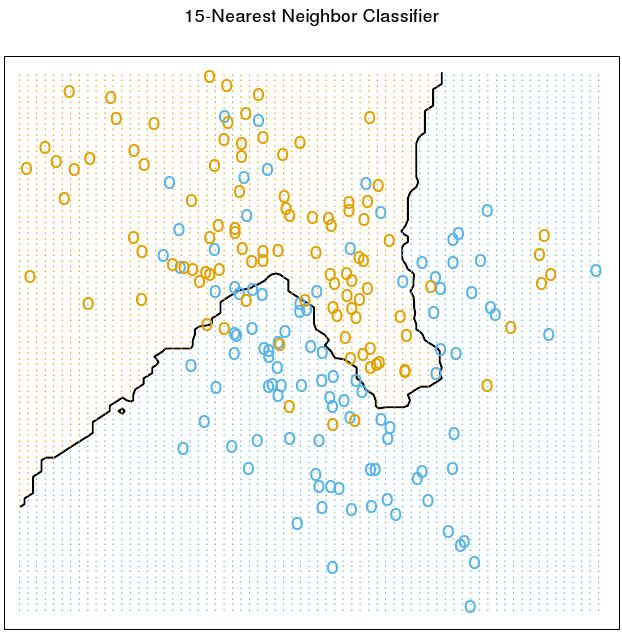
\includegraphics[width=.35\textwidth]{ex_kpp_15.jpg}
  \quad
    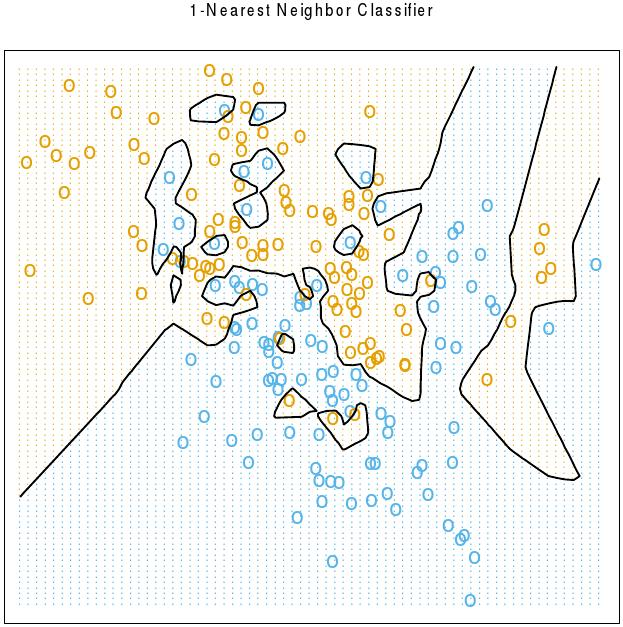
\includegraphics[width=.35\textwidth]{ex_kpp_1.jpg}\\
    $k=15$, $N_{\textrm{eff}} \approx 13$ \hspace{3cm} $k=1$, $N_{\textrm{eff}} \approx 200$
  \end{center}
  \begin{itemize}
     \item $k=1$ $\rightarrow$ training error is always $0$ !
  \end{itemize}

\end{frame}


\begin{frame}
  \frametitle{Model Selection}
  \begin{center}
    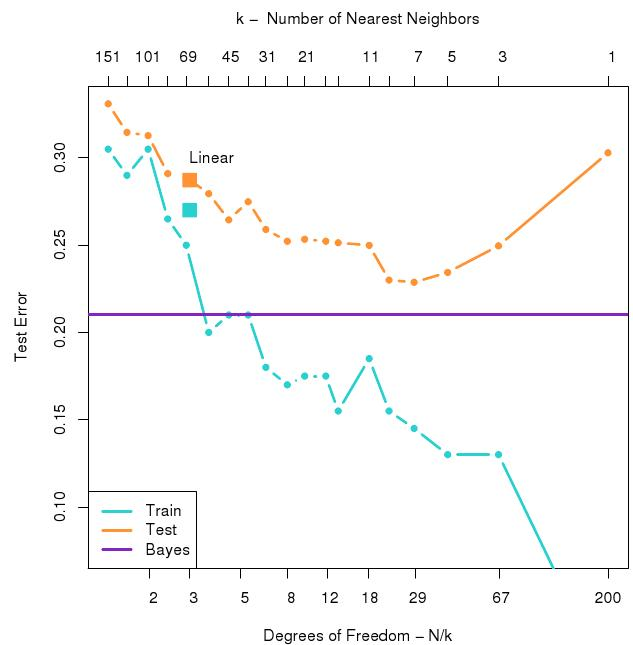
\includegraphics[width=.55\textwidth]{ex_selection_kpp_mc.jpg}
  \end{center}
\end{frame}



\subsection{Support Vector Machine (SVM)}
\begin{frame}{Support Vector Machine (SVM)}

Theory elaborated in the early 1990's (Vapnik {\em et al}) based on the idea of {\structuretext{ 'maximum margin'}}

\begin{itemize}
 \item geometrical criterion optimized on the training set $\leftarrow$  \structuretext{supervised classification}
 \item[\doigt] general, i.e. \structuretext{model free}, linear classification rule
 \item[\doigt] classification rule is linear in a transformed space of higher (possible infinite) dimension than the original input space
\end{itemize}


\end{frame}


\begin{frame}{Linear discrimination and Separating hyperplane}

  \begin{block}{Binary classification problem}
  \begin{itemize}
     \item $X \in \mathbb{R}^p$
     \item $Y \in \{-1,1\} \leftarrow $ 2 classes
     \item Training set $(x_i,y_i)$, for $i=1,\ldots,n$
  \end{itemize}
  \end{block}

 Defining a \structuretext{linear} discriminant function $h(x)$
 $\Leftrightarrow$ defining a separating \structuretext{hyperplane} $\mathcal{H}$ with equation\\
  \begin{minipage}{.4\textwidth}
\begin{center}
                   $$
 \boldsymbol{x}^T \boldsymbol{\beta} + \beta_0 = 0,
 $$
\end{center}
\end{minipage}
\quad
 \begin{minipage}{.3\textwidth}
  \begin{center}
   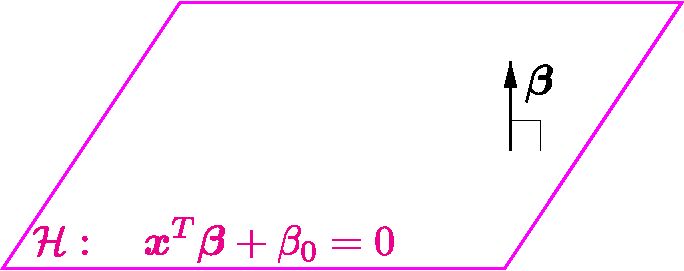
\includegraphics[width=\textwidth]{geom_hyperplane_wopoint.pdf}
  \end{center}
 \end{minipage}


\begin{itemize}
 \item $\boldsymbol{\beta} \in \mathbb{R}^p$ is the normal vector (vector normal to the hyperplane $\mathcal{H}$),
 \item $\beta_0 \in \mathbb{R}$ is the intercept/offset (regression or geometrical interpretation)
 \item[\doigt] $\mathcal{H}$ is an {\em affine subspace} of dimension $p-1$
 \item[\doigt] $h(x)\equiv \boldsymbol{x}^T \boldsymbol{\beta} + \beta_0$ is the associated (linear) discriminant function
\end{itemize}


\end{frame}





\begin{frame}{Separating hyperplane and prediction rule}

 For a given separating {hyperplane} $\mathcal{H}$ with equation \medskip \\
  \begin{minipage}{.4\textwidth}
\begin{center}
                   $$
 \boldsymbol{x}^T \boldsymbol{\beta} + \beta_0 = 0,
 $$
\end{center}
\end{minipage}
\quad
 \begin{minipage}{.3\textwidth}
  \begin{center}
   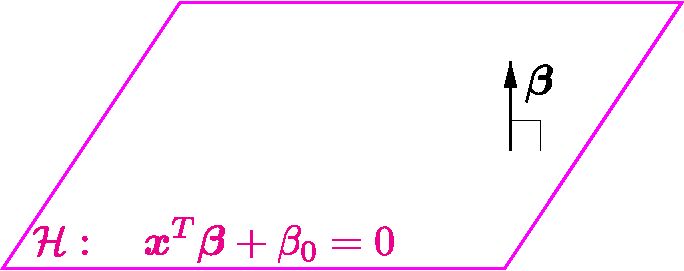
\includegraphics[width=\textwidth]{geom_hyperplane_wopoint.pdf}
  \end{center}
 \end{minipage} \bigskip \\
 the \structuretext{prediction rule} can be expressed as
\begin{itemize}
 \item $\widehat{y}=+1$, if $h(\boldsymbol{x})= \boldsymbol{x}^T \boldsymbol{\beta} + \beta_0 \ge 0$,
 \item  $\widehat{y}=-1$, otherwise,
\end{itemize}
or in an equivalent way:
\begin{align*}
 \widehat{y} &\equiv G(\boldsymbol{x}) = \structuretext{ \sign{\left[  \boldsymbol{x}^T \boldsymbol{\beta} + \beta_0 \right]} }
\end{align*}

\begin{itemize}
 \item[Rk:] $\boldsymbol{x}$ is in class  $y \in\{-1,1\}$: prediction $G(\boldsymbol{x})$ is correct %$\Leftrightarrow$
 iff $y \left(  \boldsymbol{x}^T \boldsymbol{\beta} + \beta_0 \right )  \ge 0$
 \end{itemize}

\end{frame}



%\section{Separable case}

\begin{frame}
  \frametitle{Separating Hyperplane: separable case}

  %\begin{block}{Binary supervised classification}
%   $X \in \mathbb{R}^p$, $Y \in \{-1,1\}$, Training set $(x_1,y_1),\ldots,(x_n,y_n)$
  %\end{block}

  \medskip

  \structuretext{Linear separability assumption:}
  $\exists \boldsymbol{\beta}  \in \mathbb{R}^p$ and $\beta_0 \in \mathbb{R}$ s.t. the hyperplane
  $\boldsymbol{x}^T \boldsymbol{\beta} + \beta_0 = 0$
  perfectly separates
  the two classes on the training set:
  $$\begin{displaystyle}       y_k  \left(  x^T_k \boldsymbol{\beta} + \beta_0 \right) \ge 0, \quad \textrm{ for } k=1,\ldots,n,
  \end{displaystyle}$$

%  \vspace{-2mm}
\begin{block}{Separable case ($p=2$ example)}
\begin{minipage}{.6\textwidth}
  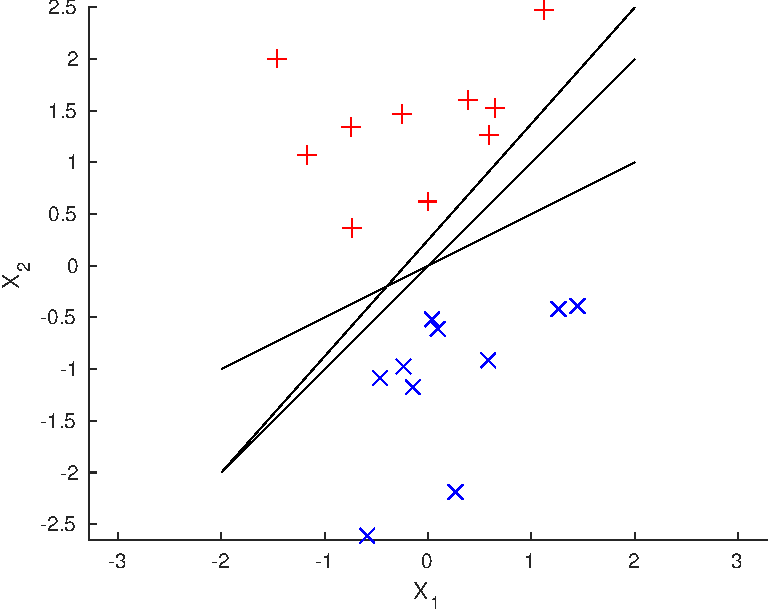
\includegraphics[width=.7\textwidth]{hyperplans_separateur.pdf}
\end{minipage}
\begin{minipage}{.39\textwidth}
  \begin{itemize}
     \item[\alert{Pb:}] infinitely \alert{many} possible perfect \alert{separating hyperplanes} $\boldsymbol{x}^T\boldsymbol{\beta} + \beta_0=0$
     \item[\doigt] Find the 'optimal' separating hyperplane
  \end{itemize}
  \end{minipage}
\end{block}

\end{frame}

\begin{frame}
   \frametitle{Maximum margin separating hyperplane (separable case)}


%    Distance of a point $\boldsymbol{x_k}$ to an hyperplane  $\mathcal{H}$ s.t. $\boldsymbol{x}^T \boldsymbol{\beta} + \beta_0 = 0$,
%    $$d(x_k,\mathcal{H}) \equiv \min_{\boldsymbol{x}} \left\{ \| \boldsymbol{x} - \boldsymbol{x}_k \| \ : \
%     \boldsymbol{x}^T \boldsymbol{\beta} + \beta_0 = 0 \right\}$$


   \begin{block}{Maximum margin principle}
   We are interested in the 'optimal' perfect separating hyperplane maximizing the distance $\structuretext{M}>0$, called the \structuretext{margin},
   between the separating hyperplane and the training data, i.e. with the biggest gap
    \end{block}
    \bigskip
   \begin{minipage}{.6\textwidth}
       \begin{center}
      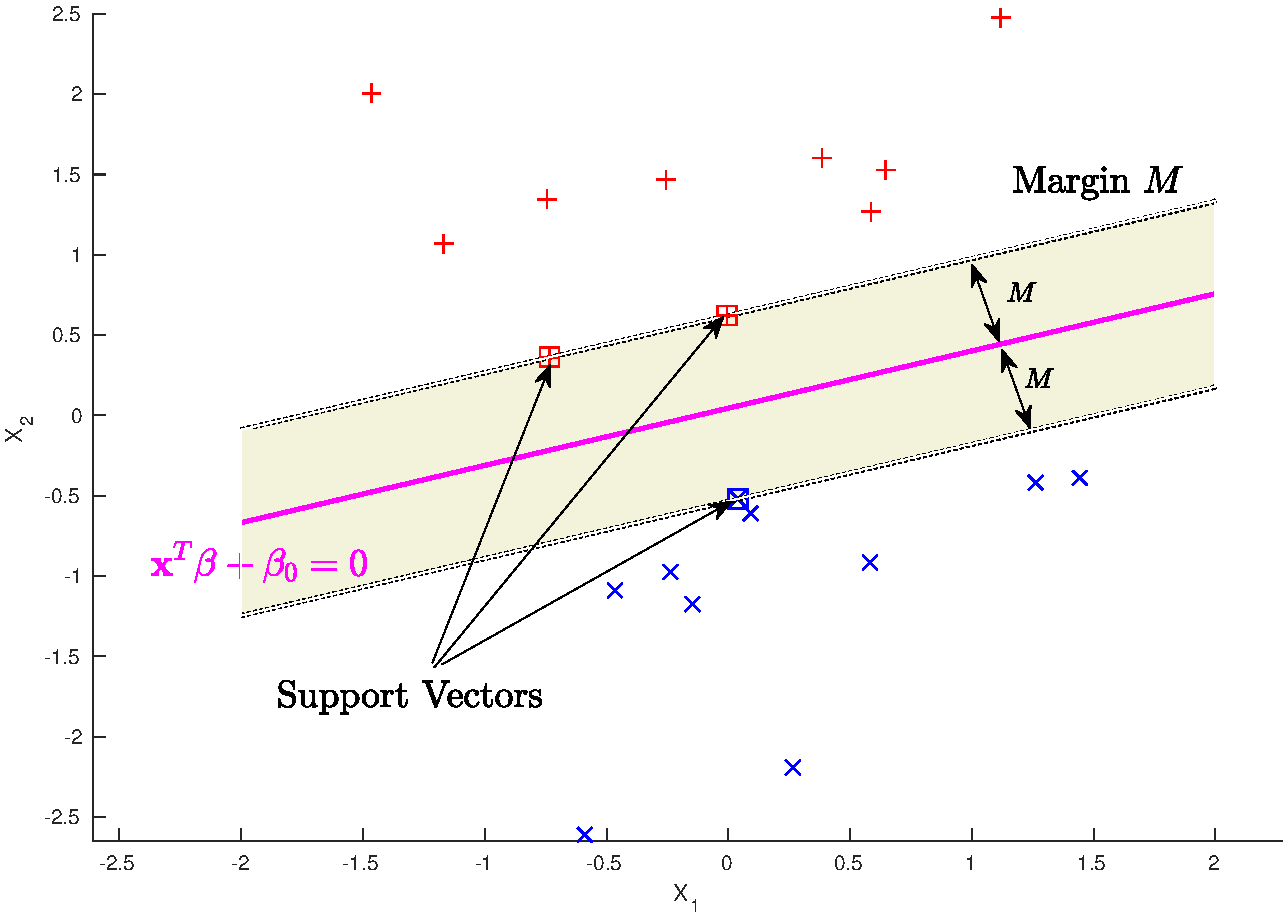
\includegraphics[width=\textwidth]{svm_margins_ann_en_DS4G.pdf}
   \end{center}
   \end{minipage}
 \begin{minipage}{.39\textwidth}
Find  $\boldsymbol{\beta}  \in \mathbb{R}^p$ and $\beta_0 \in \mathbb{R}$ s.t. the margin
    $$
      \structuretext{M}= \min_{1\le k \le n} \left\{ d(x_k,\mathcal{H}) \right\}
    $$
    is \structuretext{maximized}. Subject to
   $$\begin{displaystyle}       y_k  \left(  x^T_k \boldsymbol{\beta} + \beta_0 \right) \ge 0, \quad \text{ for } k=1,\ldots,n,
  \end{displaystyle}$$

   \end{minipage}

  \end{frame}
%
%
%   \begin{frame}
%    \frametitle{Signed distance}
%    \medskip
%
%   \begin{minipage}{.65\textwidth}
%   From the orthogonality principle,
%   $$d(x_0,\mathcal{H})=\left\|  \boldsymbol{x}_0 - \widehat{\boldsymbol{x}}_0 \right\|,$$
%   where $\widehat{\boldsymbol{x}}_0$ is the orthogonal projection of $\boldsymbol{x}_0$ on $\mathcal{H}$
% \end{minipage}
% \hfill
%  \begin{minipage}{.3\textwidth}
%   \begin{center}
%    \includegraphics[width=\textwidth]{geom_hyperplane.pdf}\\
%     $\widehat{\bx}_0 \in \mathcal{H} \Rightarrow - \widehat{\bx}_0^T\bbeta=\beta_0$
%   \end{center}
%  \end{minipage} \bigskip \\
%  \begin{itemize}
%   \item[$\Rightarrow$] $\boldsymbol{x}_0 - \widehat{\boldsymbol{x}}_0$ and  $\boldsymbol{\beta}$ are collinear,
%    \item[$\Rightarrow$] $\boldsymbol{x}_0 - \widehat{\boldsymbol{x}}_0= \underbrace{\langle \bx_0 - \widehat{\bx}_0, \bbeta^{*} \rangle}_{\textrm{signed distance}} \bbeta^{*}$, where $ \bbeta^{*}= \frac{\bbeta}{\|\bbeta\|}$, %and $\widehat{\bx}_0^T\boldsymbol{\beta} + \beta_0=0$ since $\widehat{\bx}_0 \in \mathcal{H}$
%     \item[$\Rightarrow$] $\begin{displaystyle}
%     \textrm{\structuretext{signed distance} }= \left( \bx_0 - \widehat{\bx}_0\right)^T \frac{\bbeta}{\|\bbeta\|}=
%     \frac{\bx_0^T \bbeta - \widehat{\bx}_0^T \bbeta}{\|\bbeta\|}= \structuretext{\frac{\bx_0^T \bbeta +\beta_0}{\|\bbeta\|}},\end{displaystyle}$
%  \end{itemize}
% \begin{block}{Remarks}
%   \begin{itemize}
%  %\item the last equality comes from $\widehat{\bx}_0 \in \mathcal{H}$
%     \item %$\langle \bx_0 - \widehat{\bx}_0, \bbeta^{*} \rangle\ge 0$ iff $\bx_0 - \widehat{\bx}_0$ and $\bbeta$ have same orientations, and
%     $|\langle \bx_0 - \widehat{\bx}_0, \bbeta^{*} \rangle|= \| \bx_0 - \widehat{\bx}_0 \|= d(\bx_0,\mathcal{H}) \leftarrow$  ``signed distance''
%     \item for any perfect separating hyperplane $y_k \langle \bx_k - \widehat{\bx}_k, \bbeta^{*} \rangle= \frac{1}{\|\bbeta\|} y_k ( \bx_k^T \bbeta +\beta_0)  \ge 0$, for $k=1,\ldots,n$,
%  \end{itemize}
%      \end{block}
%   \end{frame}
%
%
%     \begin{frame}
%    \frametitle{Canonical separating hyperplane}
%
%    For any perfect separating hyperplane, for  $k=1,\ldots,n$
%    $$y_k \langle \bx_k - \widehat{\bx}_k, \bbeta^{*} \rangle= d(x_k,\mathcal{H})$$
%    Hence, the
%    margin reads
%    $$
%    M \equiv \min_{1\le k\le n} \left\{  d(x_k,\mathcal{H}) \right\} =  \frac{1}{\| \bbeta \| } \min_{1\le k\le n} \left\{ y_k ( \bx_k^T \bbeta +\beta_0)  \right\}
%    $$
%
%    \begin{block}{Remarks}
%     \begin{itemize}
%      \item The bound $M$ is reached (min of a countable set),
%      \item[\doigt] the samples at the margin are denoted as $\bx_{\textrm{margin}}$
%     \end{itemize}
% \end{block}
% \begin{block}{Canonical expression of the separating hyperplane}
%  $\bbeta$ and $\beta_0$ are normalized s.t.
%      $$
%      y_{\textrm{margin}} ( \bx_{\textrm{margin}}^T \bbeta +\beta_0) =1, \quad
%    \textrm{thus }
%      \structuretext{M=\frac{1}{\| \bbeta \|}}
%      $$
%    \end{block}
% \end{frame}

%
%
% \begin{frame}
%    \frametitle{Optimization problem (separable case)}
%    \begin{minipage}{.6\textwidth}
%        \begin{center}
%       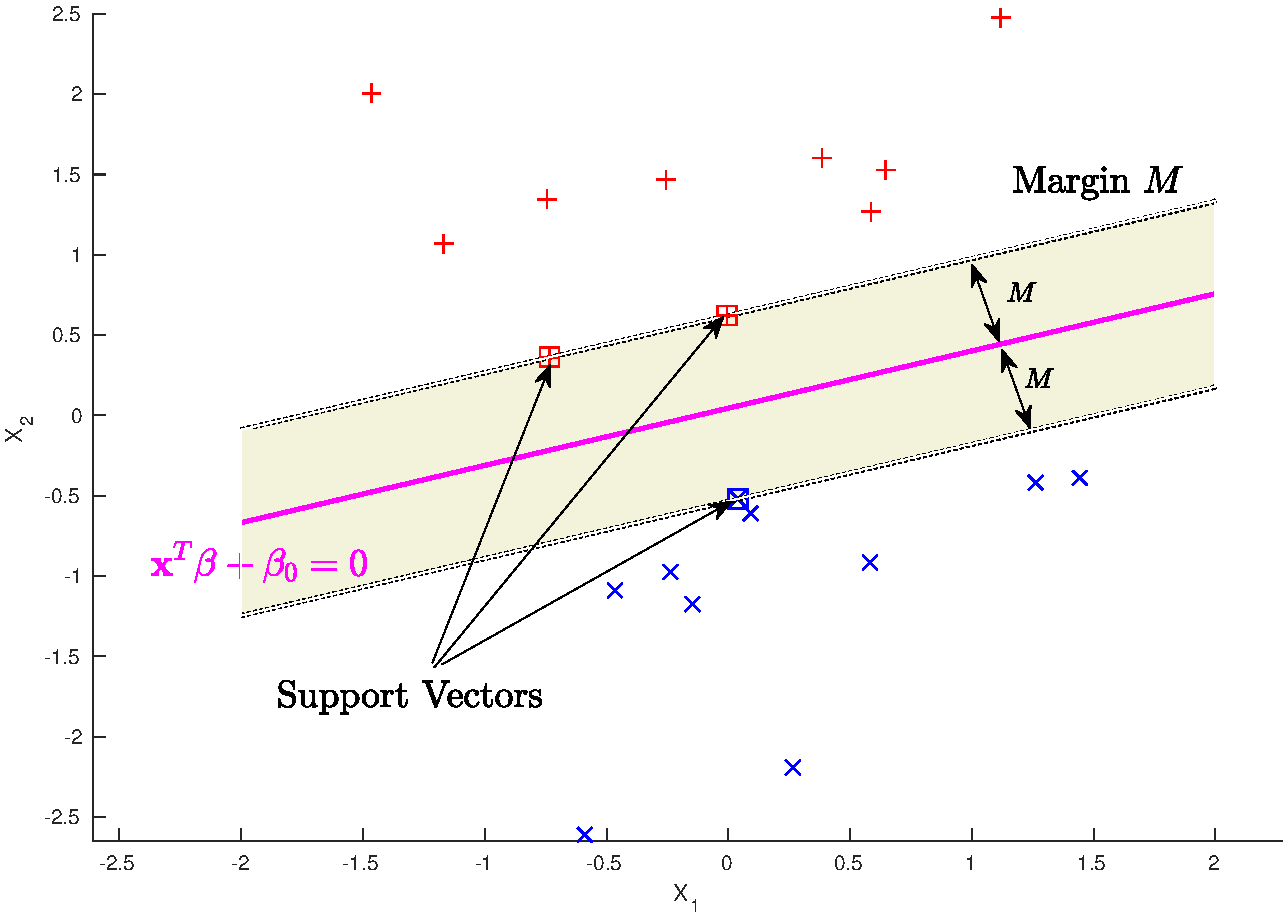
\includegraphics[width=\textwidth]{svm_margins_ann_en_DS4G.pdf}
%    \end{center}
%    \end{minipage}
%  \begin{minipage}{.39\textwidth}
%
%    %\begin{block}{Primal optimization problem}
%    $$\left\{ \begin{array}{lc}
%     \max_{\bbeta,\beta_0}    & M,\\
%     \textrm{subject to } &y_k \left( \bx_k^T \bbeta + \beta_0 \right) \ge 1,\\ & \textrm{ for } 1 \le k \le n.
%    \end{array}\right. $$
%    \end{minipage}
%
% \begin{itemize}
%  \item can be recast as a quadratic criterion + linear inequality  constraints
%  \item[\doigt] simple convex optimization problem for which standard numerical procedure are available
%    \item[\doigtr] the only \alert{inputs used to construct the maximum margin hyperplane} are the  \alert{support vectors}
%  \end{itemize}
%
%     %Minimizing $\begin{displaystyle} \frac{1}{2} \|\bbeta\|^2 \end{displaystyle}$\\
%  %  \end{block}
%
%
% \end{frame}
%
% \begin{frame}
%    \frametitle{Lagrangian (separable case)}
%
%    Convex constraints of positivity $\Rightarrow$ introduction of the Lagrange multipliers
%    \begin{block}{Lagrangian}
%     $$ L(\bbeta,\beta_0,\balpha) = \frac{1}{2} \|\bbeta\|^2 - \sum_{i=1}^n \alpha_i
%     \underbrace{\left[ y_i ( \bx_i^T \bbeta + \beta_0 )-1\right]}_{\ge 0},$$
%     where $\alpha_i$ are the Lagrange multipliers
%    \end{block}
%
%
%    \begin{block}{First order Kuhn-Tucker necessary conditions}
%    Setting the partial derivatives w.r.t. $\bbeta$ and $\beta_0$ to zero yields
%    $$\left\{ \begin{array}{ll}
%     \widehat{\bbeta}& = \sum_{i=1}^n \alpha_i y_i \bx_i,\\
%     0 &=  \sum_{i=1}^n \alpha_i y_i,
%     \end{array}\right. $$
%     \begin{itemize}
%      \item plugging these expression in the Lagrangian yields the dual expression
%     \end{itemize}
%
%    \end{block}
%
%
% \end{frame}
%
%
% \begin{frame}
%    \frametitle{Dual problem (separable case)}
%
%
%       \begin{block}{Dual optimization problem}
%    $$\left\{ \begin{array}{lc}
%     \max_{\balpha}    & \widetilde{L}(\balpha)  =  \sum_{i=1}^n \alpha_i  - \frac{1}{2}   \sum_{i,j=1}^n \alpha_i \alpha_j y_i y_j
%     \bx_i^T \bx_j,\\
%     \textrm{subject to } & \alpha_i \ge 0 \textrm{ and } \sum_{i=1}^n \alpha_i y_i= 0.
%    \end{array}\right. $$
%
% \begin{itemize}
%  \item[\doigt]  simple convex optimization problem for which standard numerical procedure are available
%  \item[\doigt] calculation of the optimum multipliers $\widehat{\alpha}_i$
% \end{itemize}
%    \end{block}
%
%
%
% \end{frame}
%
%
% \begin{frame}
%    \frametitle{Support vectors and  maximum margin hyperplane (separable case)}
%
%
%
%    \begin{block}{Complementary slackness Kuhn-Tucker necessary conditions}  % \vspace{-2.5mm}
%    $$\widehat{\alpha}_i [ y_i h(\bx_i) -1]=0 \quad \Rightarrow \quad \structuretext{ \widehat{\alpha}_i=0  \ \textrm{  as  } \ y_i h(\bx_i) >1}$$
%   %\vspace{-4mm}
%    \begin{itemize}
%  \item since  $\widehat{\bbeta} = \sum_{i=1}^n \widehat{\alpha}_i y_i \bx_i$,  $\widehat{\bbeta}$ depends only on the points at the margin $\leftarrow$ \structuretext{support vectors}
%  \item $\widehat{\beta}_0$ can be derived from the  complementary slackness expression for any of support vectors $\bx_{\textrm{margin}}$
%  $$\begin{array}{lll}
%      y_{\textrm{margin}} h( \bx_{\textrm{margin}} ) - 1  = 0&
%      \Rightarrow & \widehat{\bbeta}^T \bx_{\textrm{margin}} + \widehat{\beta}_0 = y_{\textrm{margin}},\\
%      & \Rightarrow & \widehat{\beta}_0 = -\widehat{\bbeta}^T \bx_{\textrm{margin}} +  y_{\textrm{margin}}
%    \end{array}$$
%  \item[\doigtr] the only \alert{inputs used to construct the maximum margin hyperplane} are the  \alert{support vectors} and the discriminant function reads
%  $$h(\bx)= \sum_{i=1}^n \widehat{\alpha}_i y_i (\bx- \bx_{\textrm{margin}})^T \bx_i +  y_{\textrm{margin}}$$
%  \end{itemize}
%   \end{block}
%
%
% \end{frame}
%
%
%
%   \begin{frame}
%    \frametitle{Maximum margin separating hyperplane (separable case)}
%
%        \begin{block}{Separable case}
%       \begin{itemize}
%       \item[\doigt] Maximizing the  {\em margin} $M$ between the
%       separating hyperplane and the training data:
%       %$ y_i(\boldsymbol{x_i}^T \boldsymbol{\beta} + \beta_0) \ge M$
%       \end{itemize}
%     \end{block}
%
%    \begin{center}
%       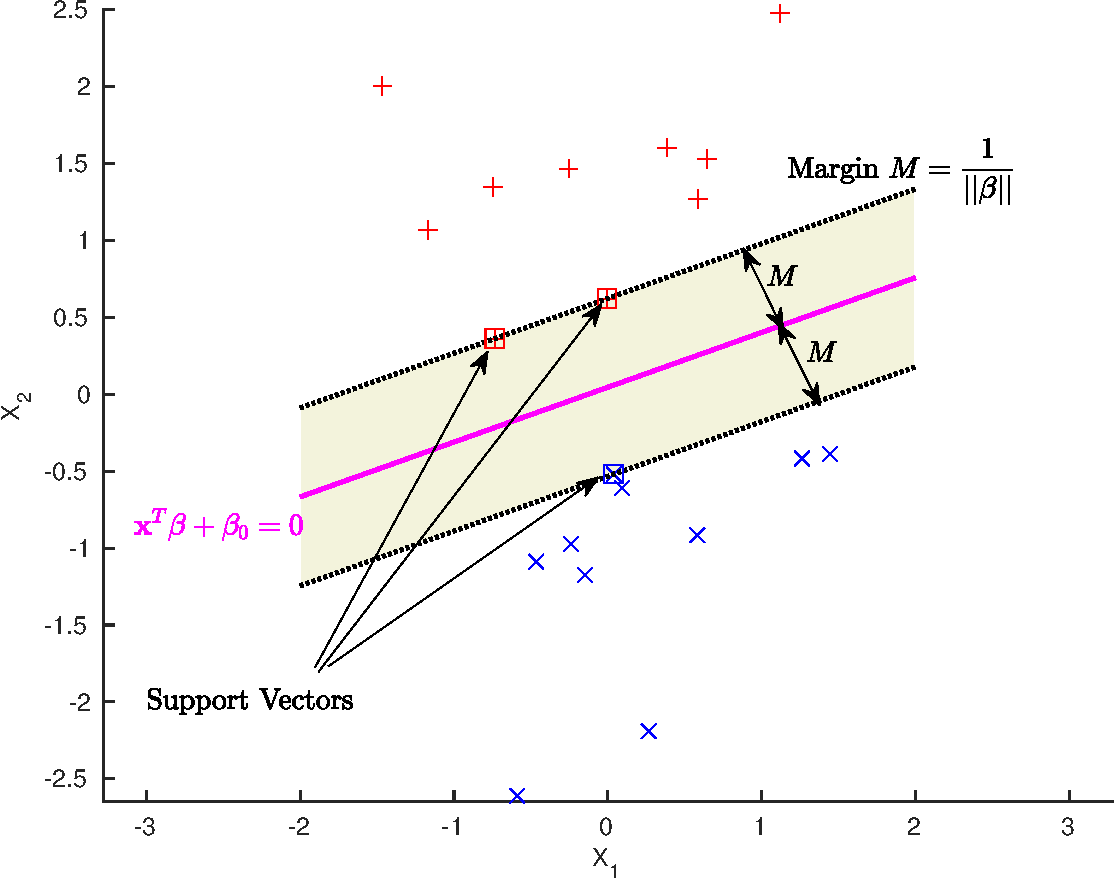
\includegraphics[width=.7\textwidth]{svm_margins_ann_en.pdf}
%    \end{center}
%    \begin{itemize}
%      \item[\doigtr] the only \alert{inputs used to construct the maximum margin hyperplane} are the
%      \alert{support vectors} and the discriminant function
%    \end{itemize}
%
% \end{frame}

%\section{Nonseparable case}

\begin{frame}
   \frametitle{Nonseparable case}
   \begin{block}{}
      \begin{itemize}
      \item in general, overlap of the 2 classes (unless $n<p$)
      \item no hyperplane that perfectly separates the training data
      \end{itemize}
    \end{block}

   \begin{center}
      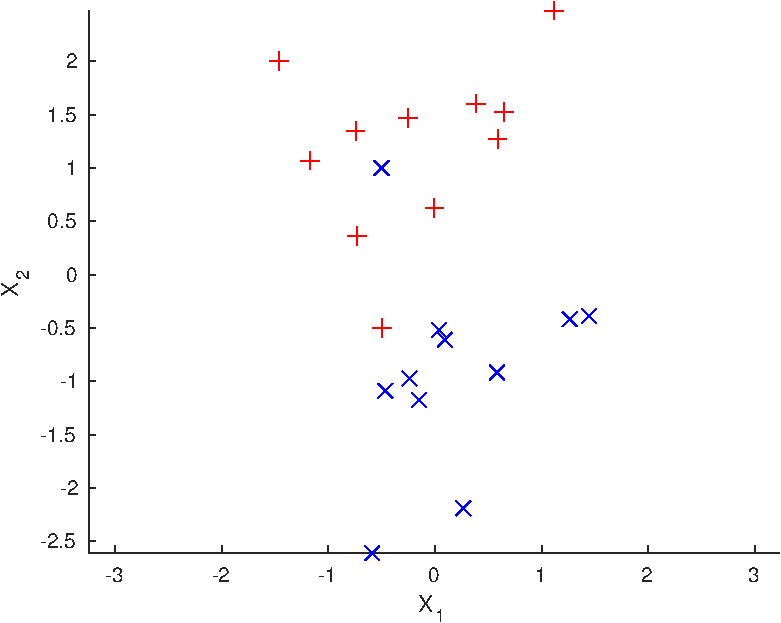
\includegraphics[width=.45\textwidth]{nonsep_svm_pb.pdf}
   \end{center}
     \begin{itemize}
      \item[\doigtr] we can soften what we mean by ``separates''
      \end{itemize}
\end{frame}


\begin{frame}
   \frametitle{Maximum margin separating hyperplane (nonseparable case)}
   \begin{block}{Solution for the nonseparable case}
   Considering a {\em soft-margin} that allows  wrong classifications
      \begin{itemize}
      \item introduction of {\em slack variables} $\xi_i\ge 0$ s.t.
     \begin{align*}
         y_i(\boldsymbol{x_i}^T \boldsymbol{\beta} + \beta_0) & \ge (1-\xi_i)
      \end{align*}
      Support vectors include now the wrong classified points, and the points inside the margins ($\xi_i > 0$)
     \item Primal problem: adding a constraint on the $\xi_i$'s
     $$\left\{ \begin{array}{ll}
       \max_{\bbeta,\beta_0,\xi} & M,\\
       \textrm{subject to } &   y_i(\boldsymbol{x_i}^T \boldsymbol{\beta} + \beta_0)  \ge 1 \alert{-\xi_i}, \\
       & C\, \sum_{i=1}^n \xi_i \le 1.
      \end{array} \right.$$
      where $C>0$ is the ``cost'' parameter
      \end{itemize}
    \end{block}

\end{frame}


% \begin{frame}
%    \frametitle{Cost parameter (nonseparable case)}
%         $$
%          \textrm{Criterion to be minimized: } \quad \frac{1}{2} || \boldsymbol{\beta}||^2 + C \sum_{i=1}^n \xi_i,
%       $$
%    \begin{block}{Influence of the cost parameter $C>0$}
%  $C$ drives the margin size, thus the number of support vectors
%        \begin{itemize}
%          \item $C \gg 0$~: $\sim$ underfitting (small margin, less support vectors)
%          \item $C \rightarrow 0^+$~: $\sim$ overfitting (large margin, more  support vectors)
%          \item $C \rightarrow +\infty$~: converges to the separable case
%        \end{itemize}
%        %\item $\xi_i^* = M \xi_i \leftarrow$ distance between a support vector and the margin
%     \end{block}
%
%     \begin{block}{Choosing the cost parameter $C>0$}
%      \begin{itemize}
%          \item the optimal $C$ can be estimated by cross validation
%          \item[\doigt] performance might not be very sensitive to choices of $C$ (because of the rigidity of a linear boundary)
% 	 \item[\doigt] usually $C\approx 1$ yields a good trade-off
%        \end{itemize}
%     \end{block}
%
%
% \end{frame}
%
% \begin{frame}
%    \frametitle{Dual problem (nonseparable case)}
%
%    Introducing the Lagrangian and substituting the first order KT conditions w.r.t. $\bbeta$, $\beta_0$, $\bxi$
%    yields the dual expression
%     \begin{block}{Dual optimization problem}
%    $$\left\{ \begin{array}{lc}
%     \max_{\balpha}    & \widetilde{L}(\balpha)  =  \sum_{i=1}^n \alpha_i  - \frac{1}{2}   \sum_{i,j=1}^n \alpha_i \alpha_j y_i y_j
%     \bx_i^T \bx_j,\\
%     \textrm{subject to } & 0 \le  \alpha_i \alert{\le C} \textrm{ and } \sum_{i=1}^n \alpha_i y_i= 0.
%    \end{array}\right. $$
%
% \begin{itemize}
%  \item[\doigt] only difference w.r.t the separable case: $\alpha_i \alert{\le C}$ constraint!
%  \item[\doigt]  simple convex optimization problem for which standard numerical procedure are available
% \end{itemize}
%  \end{block}
%
% \end{frame}
%

\begin{frame}
   \frametitle{Optimal separating hyperplane}
    \begin{block}{Example (nonseparable case)}
    \end{block}
 \begin{minipage}{.65\textwidth}
     \begin{center}
      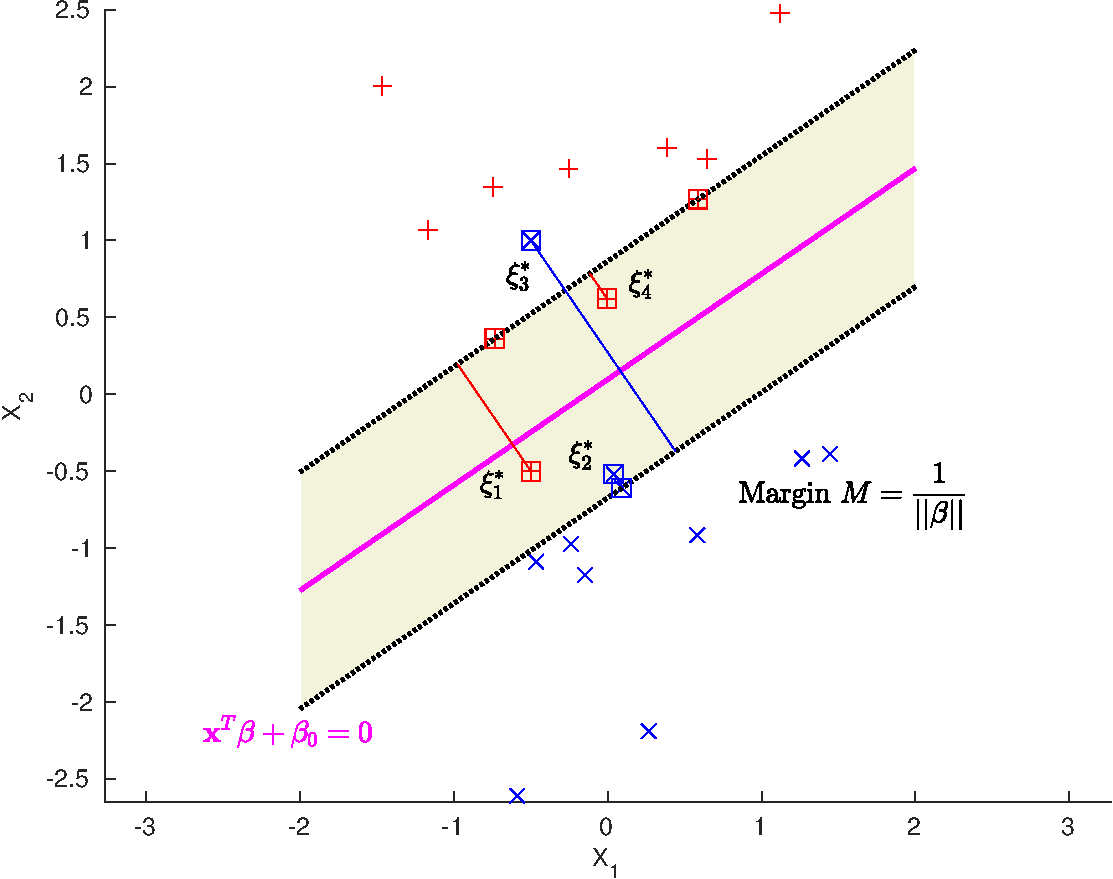
\includegraphics[width=\textwidth]{nonsep_svm_ann_en.pdf}
   \end{center}
 \end{minipage} \hfill
\begin{minipage}{.33\textwidth}
%\begin{center}
                 $\xi_i^* \equiv M \xi_i \leftarrow$ distance between a support vector and the margin
%                \end{center}
\end{minipage}


\end{frame}


%\section{Linear discrimination: comparison of SVM vs LDA}

\begin{frame}
  \frametitle{Linear discrimination:  SVM vs LDA}
  \begin{block}{Linear discrimination}
   \begin{itemize}
    \item Linear Discriminant Analysis (LDA): Gaussian generative model
    \item SVM: criterion optimization (maximizing the margin)
   \end{itemize}
  \end{block}


\begin{minipage}{.48\textwidth}
\begin{center}
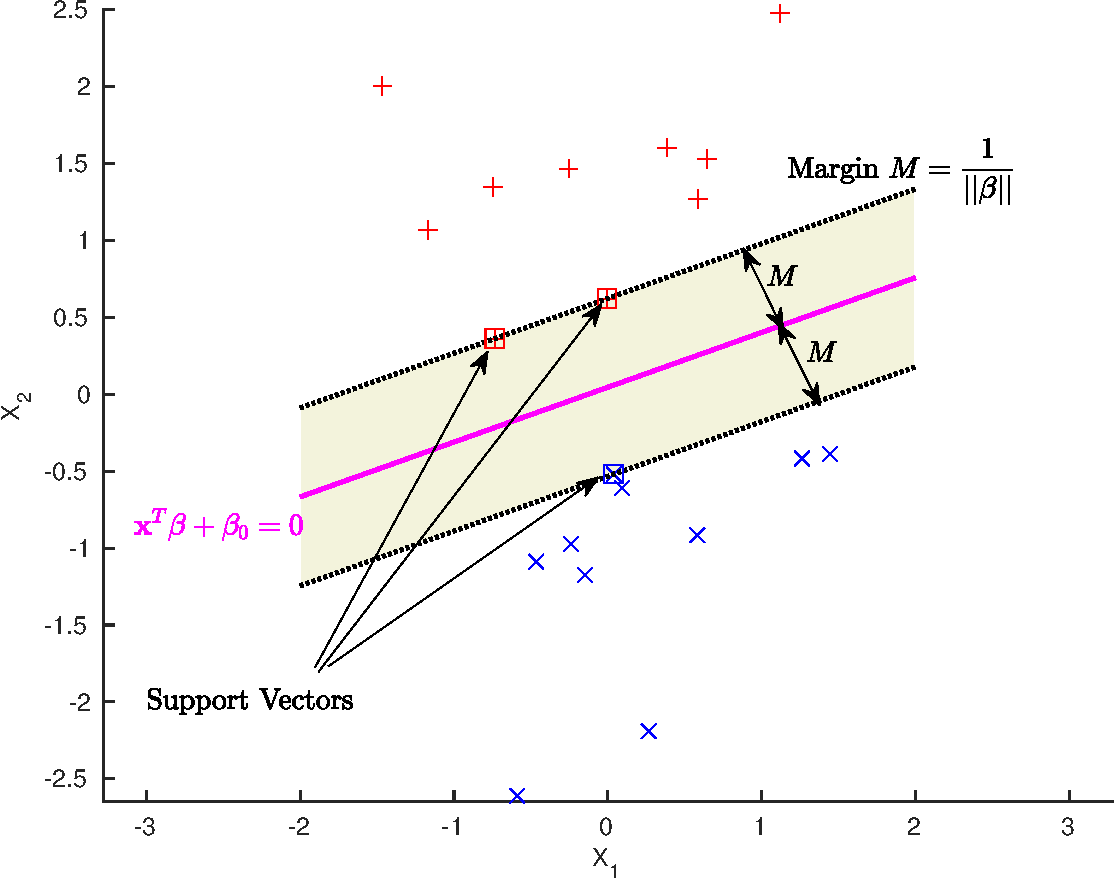
\includegraphics[height=40mm]{svm_margins_ann_en.pdf}\\
\textcolor{blue}{SVM}
\end{center}
\end{minipage}
\hfill
\begin{minipage}{.48\textwidth}
\begin{center}
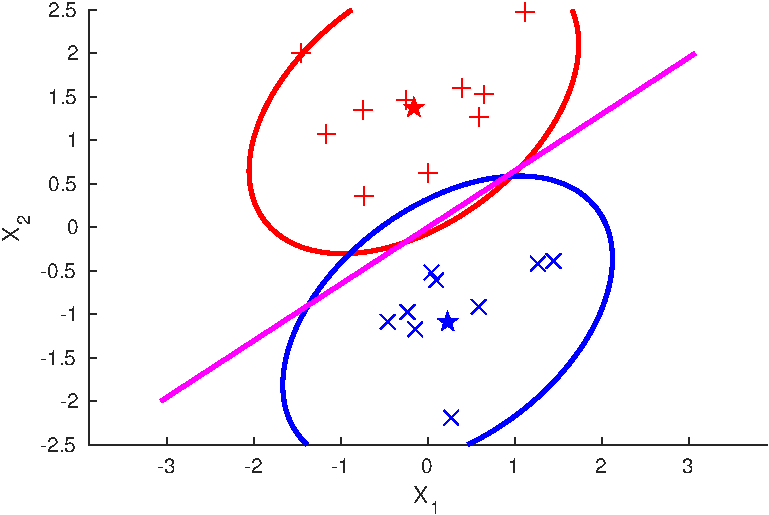
\includegraphics[height=41mm]{lda.pdf}\\
\textcolor{blue}{LDA}
\end{center}
\end{minipage}

\end{frame}


\begin{frame}
  \frametitle{Linear discrimination:  SVM vs LDA (Cont'd)}

\begin{block}{Adding one atypical data}
\end{block}


\begin{minipage}{0.35\textwidth}
\begin{center}
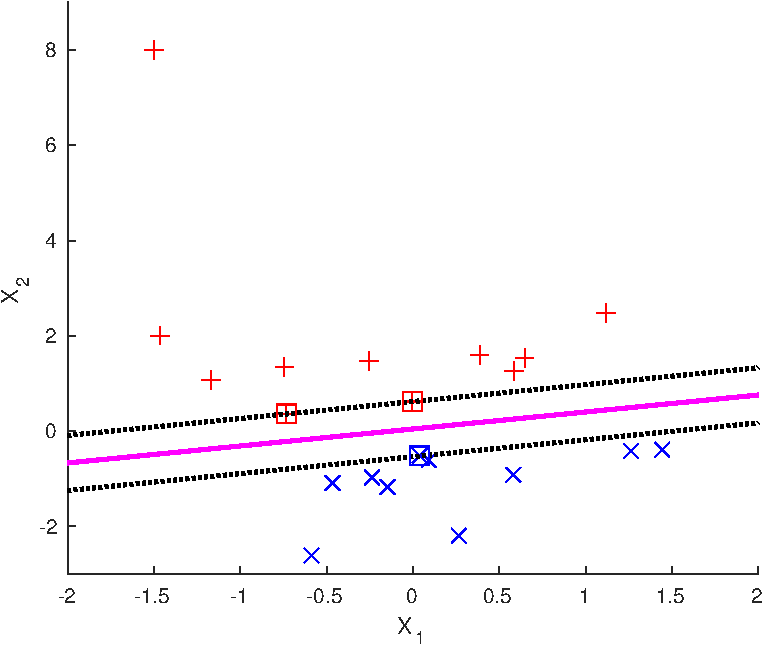
\includegraphics[width=\textwidth]{svm_margins_out.pdf}\\
\textcolor{blue}{SVM}
\end{center}
\end{minipage}
\hfill
\begin{minipage}{0.35\textwidth}
\begin{center}
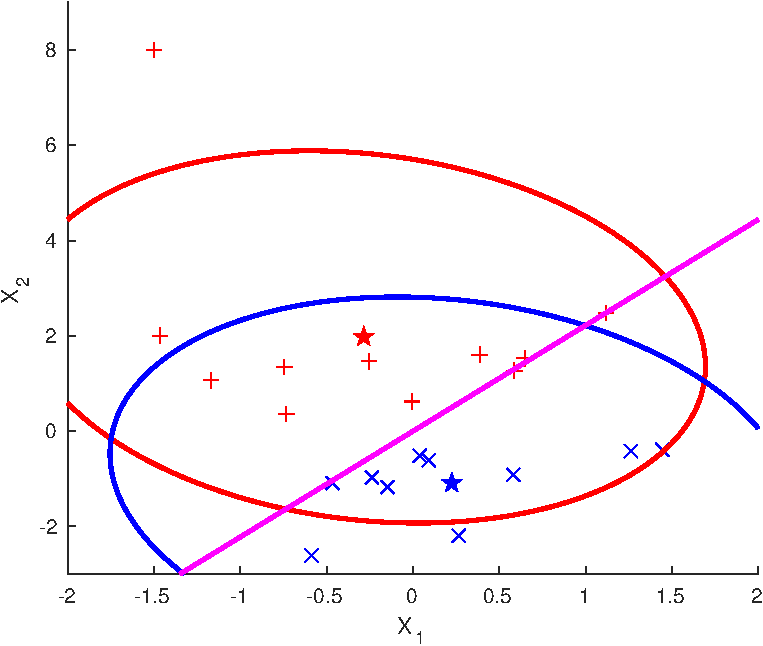
\includegraphics[width=\textwidth]{lda_out.pdf}\\
\textcolor{blue}{LDA}
\end{center}
\end{minipage}

  \begin{block}{SVM property}
   \begin{itemize}
    \item Nonsensitive to atypical points (outliers) far from the margin
    \item[\doigt] sparse method (information $\equiv$ support vectors)
   \end{itemize}
  \end{block}

\end{frame}

\begin{frame}
  \frametitle{Nonlinear discrimination in the input space}


\begin{center}
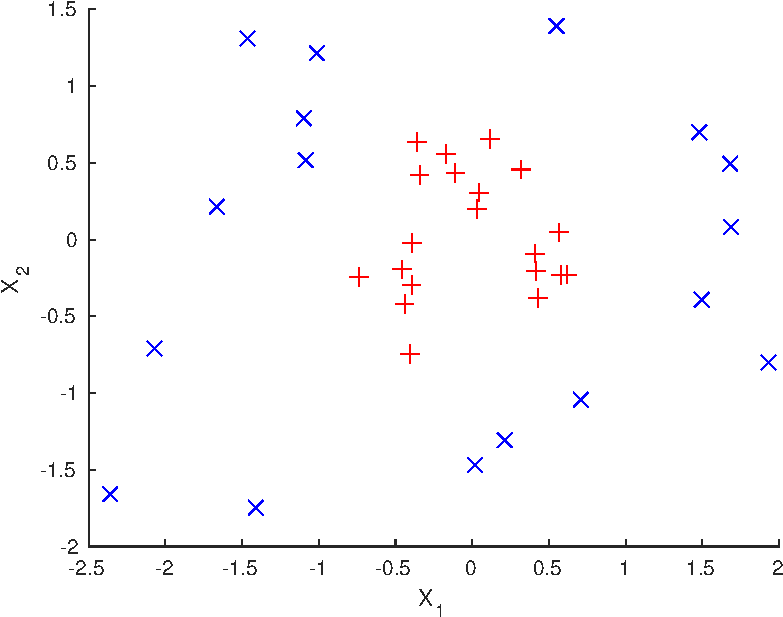
\includegraphics[width=.4\textwidth]{non_lin_pb.pdf}
\end{center}

\begin{block}{Transformed space $\mathcal{F}$}
\begin{itemize}
   \item Choice of a transformed space  $\mathcal{F}$ (expansion space) where
   the linear separation assumption is more relevant
   \item Nonlinear expansion map $\phi~: \mathbb{R}^p \rightarrow \mathcal{F} $, $\bx\mapsto \phi(\bx)$ (enlarged features)
\end{itemize}


\end{block}


\end{frame}

\begin{frame}{Nonlinear discrimination in the input space}
  \begin{itemize}
  \item Projection in the space of monomials of order 2.
    \begin{align*}
      \phi :\mathbb{R}^2  & \to  \mathbb{R}^3\\
      \mathbf{x}          & \mapsto   \phi(\mathbf{x})\\
      (\mathbf{x}_1,\mathbf{x}_2)           & \mapsto  (\mathbf{x}_1^2,\mathbf{x}^2_2,\sqrt{2}\mathbf{x}_1\mathbf{x}_2)
    \end{align*}

  \item  In \(\mathbb{R}^3\), the inner product can be expressed as
    \begin{align*}
      \langle \phi(\mathbf{x}),\phi(\mathbf{x}')\rangle_{\mathbb{R}^3}&=   \sum_{\scriptscriptstyle i=1}^{\scriptscriptstyle 3}\phi(\mathbf{x})_i\phi(\mathbf{x}')_i \\
                                                                      &= \phi(\mathbf{x})_1\phi(\mathbf{x}')_1 + \phi(\mathbf{x})_2\phi(\mathbf{x}')_2 + \phi(\mathbf{x})_3\phi(\mathbf{x}')_3\\
                                                                      &= \mathbf{x}_1^2\mathbf{x'}_1^2 + \mathbf{x}_2^2\mathbf{x'}_2^2 + 2\mathbf{x}_1\mathbf{x}_2\mathbf{x'}_1\mathbf{x'}_2\\
                                                                      &= (\mathbf{x}_1\mathbf{x'}_1 + \mathbf{x}_2\mathbf{x'}_2)^2\\
                                                                      &= \langle \mathbf{x},\mathbf{x}'\rangle_{\mathbb{R}^2}^2\\
                                                                      &= k(\mathbf{x},\mathbf{x}').\\
      \end{align*}
      \end{itemize}

\end{frame}


\begin{frame}
  \frametitle{Nonlinear discrimination in the input space}

\begin{itemize}
 \item  $X \in \mathbb{R}^2$, $\phi(x)= (x_1^2,x_2^2,\sqrt{2}x_1 x_2)^T$
\end{itemize}

\begin{center}
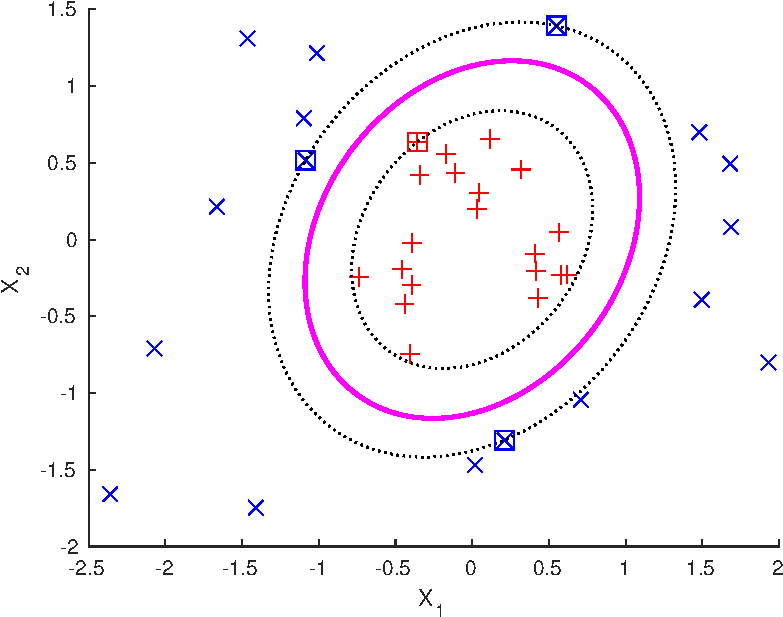
\includegraphics[width=.55\textwidth]{nonlinear_svm.pdf}\\
\color{blue}{Linear separation in the feature space $\mathcal{F}$ $\Rightarrow$
Nonlinear separation in the input space}
\end{center}


\end{frame}



\begin{frame}
  \frametitle{Kernel trick}

The SVM solution depends only on the \structuretext{inner product} between the input features $\phi(\bx)$ and the support vectors
  $\phi(\bx_{\textrm{margin}})$

  \begin{block}{Kernel trick}
  Use of  a kernel function $k$ associated with an expansion/feature map $\phi$:
  $$\begin{array}{ccll} k:& \mathbb{R}^p \times \mathbb{R}^p  &\rightarrow& \mathbb{R}\\
              & (\bx,\bx') &\mapsto& \structuretext{ k (\bx,\bx') \equiv \langle \phi(\bx), \phi(\bx') \rangle}
             \end{array}$$
  %and the separating hyperplane reads $h(\bx)= \sum_{i=1}^n \widehat{\alpha}_i y_i k(\bx_i,\bx)+ \widehat{\beta}_0$
  \end{block}

 \begin{block}{Advantages}
  \begin{itemize}
   \item Computations are performed in the original input space: less  expansive than in a high
   dimensional transformed space $\mathcal{F}$
   \item Explicit representations of the feature map $\phi$ and enlarged feature space $\mathcal{F}$ are not necessary, the only expression of $k$
   is required!
   \item[\doigt] Possibility of complex transformations in possible infinite space  $\mathcal{F}$
   \item[\doigt] \structuretext{Standard trick} in machine learning not limited to SVM (kernel ridge regression, gaussian process, kernel-PCA, spectral clustering $\ldots$)
  \end{itemize}

 \end{block}


\end{frame}

\begin{frame}{Kernel function}
  \begin{definition}[Positive semi-definite kernel]
\(k:\mathbb{R}^d\times\mathbb{R}^d   \to    \mathbb{R}\)   is   positive
semi-definite is
\begin{itemize}
\item \(\forall (\mathbf{x},\mathbf{x}')\in\mathbb{R}^d\times\mathbb{R}^d,
  k(\mathbf{x}_i,\mathbf{x}_j)=k(\mathbf{x}_j,\mathbf{x}_i)\).
\item \(\forall   n\in\mathbb{N},\forall  \xi_1\ldots\xi_n   \in\mathbb{R},
  \forall     \mathbf{x}_1\ldots\mathbf{x}_n      \in     \mathbb{R}^d,
  \sum_{i,j}^n\xi_i\xi_jk(\mathbf{x}_i,\mathbf{x}_j)\geq 0\).
\end{itemize}
\end{definition}

\begin{theorem}[Moore-Aronsjan (1950)]
To every  positive semi-definite  kernel \(k\),  there exists  a Hilbert
space        \(\mathcal{H}\)       and        a       feature        map
\(\phi:\mathbb{R}^d\to\mathcal{H}\)      such      that     for      all
\(\mathbf{x}_i,\mathbf{x}_j\)  we  have \(k(\mathbf{x}_i,\mathbf{x}_j)  =
\langle\phi(\mathbf{x}_i),\phi(\mathbf{x}_j)\rangle_\mathcal{H}\).
\end{theorem}

\end{frame}
\begin{frame}[label={sec:orgheadline17}]{Operations on kernels}
Let \(k_1\)  and \(k_2\) be positive  semi-definite, and \(\lambda_{1,2}>0\)
then:
\begin{enumerate}
\item \(\lambda_1k_1\) is a valid kernel
\item \(\lambda_1k_1+\lambda_2k_2\) is positive semi-definite.
\item \(k_1k_2\) is positive semi-definite.
\item \(\exp(k_1)\) is positive semi-definite.
\item \(g(\mathbf{x}_i)g(\mathbf{x}_j)\)  is  positive  semi-definite,  with
\(g:\mathbb{R}^d\to\mathbb{R}\).
\end{enumerate}
\end{frame}

\begin{frame}
  \frametitle{Choosing the Kernel function}

%  \begin{block}{Mercer theorem}
%  $k(\cdot,\cdot)$ should be a symmetric positive (semi-) definite function
%  \end{block}

  \begin{block}{Usual kernel functions}
\begin{itemize}
 \item  Linear kernel ( $\mathcal{F} \equiv \mathbb{R}^p$)~:
 $
    k(x,x') =x^T x'
$
 \item  Polynomial kernel (dimension of $\mathcal{F}$ increases with the order $d$)
 \begin{align*}
    k(x,x') &=(x^T x'+q)^d = \sum_{l=1}^d\binom{d}{l}q^{d-l}(x^Tx')^l.
 \end{align*}
  \item Gaussian radial function ($\mathcal{F}$ with infinite dimension)
 \begin{align*}
    k(x,x') &= \exp{\left( - \gamma ||x - x'||^2\right)}
 \end{align*}
   \item  Neural net kernel ($\mathcal{F}$ with infinite dimension)
 \begin{align*}
    k(x,x') &= \tanh{\left( \kappa_1 x^T x' + \kappa_2 \right)}
 \end{align*}
\item[\doigt] standard practice is to estimate optimal values of kernel parameters  by \structuretext{cross validation}
\end{itemize}
 \end{block}

\end{frame}


\begin{frame}
  \frametitle{Application: binary data  (cf introduction course)}

  \begin{block}{Linear kernel}
    \begin{center}
      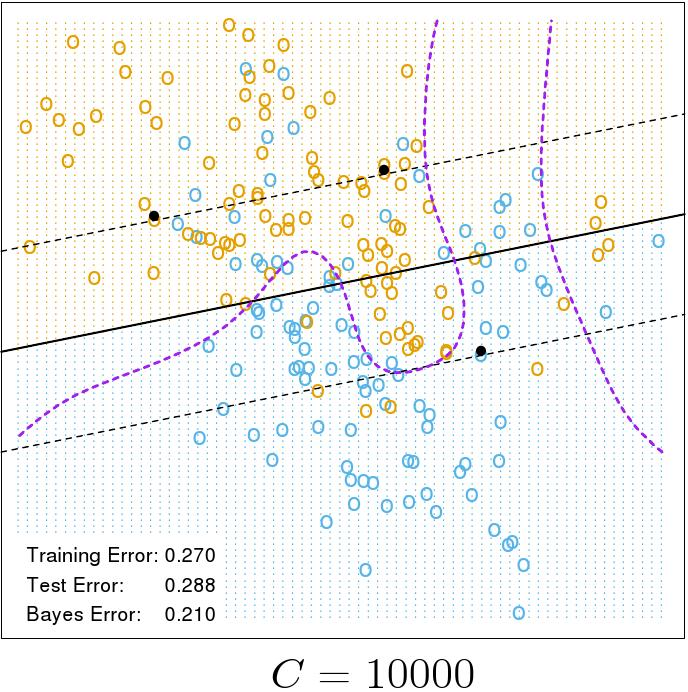
\includegraphics[trim=0 30 0 0,clip,width=.45\textwidth, ]{exempleBin_lin1.jpg}%\\
      % \color{blue}{$C=10000$}
    \end{center}
  \end{block}
\end{frame}

\begin{frame}
  \frametitle{Application: binary data}


  \begin{block}{Polynomial kernel ($d=4$)}
    \begin{center}
      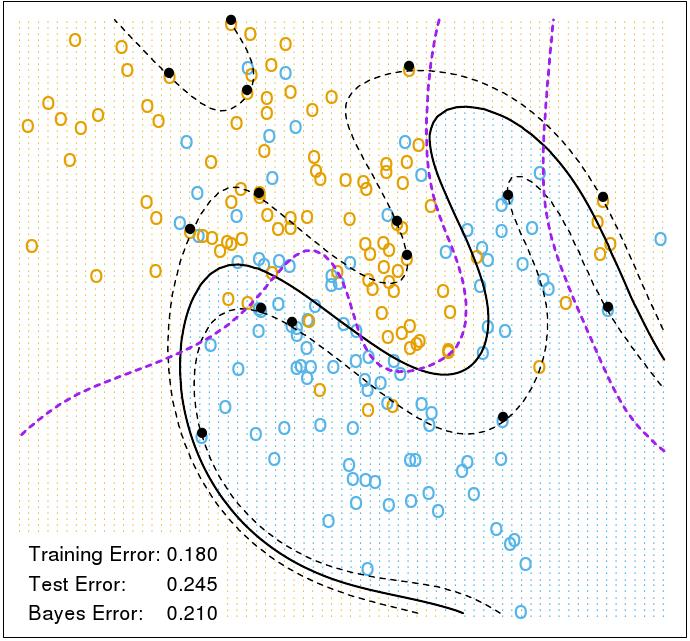
\includegraphics[width=.45\textwidth]{exempleBin_poly4.jpg}\\
      % \color{blue}{$C \approx 1$}
    \end{center}

  \end{block}
\end{frame}


\begin{frame}
  \frametitle{Application: binary data}

  \begin{block}{Gaussian radial kernel ($\gamma=1$)}
    \begin{center}
      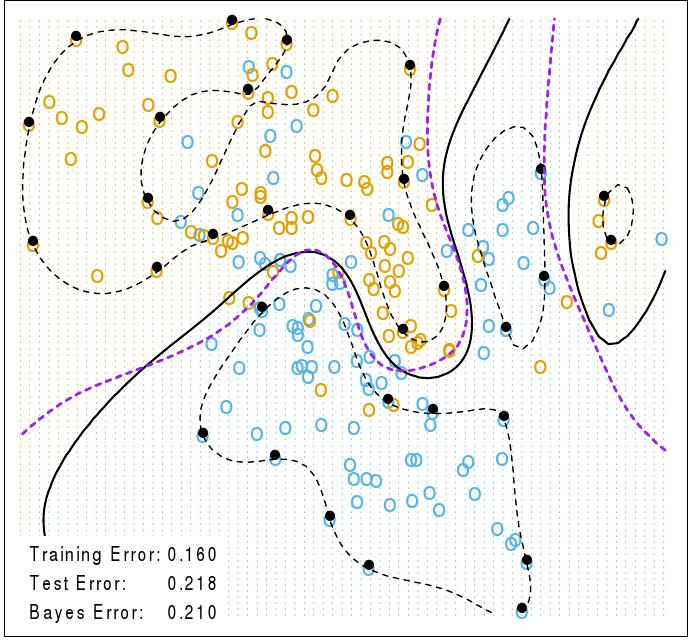
\includegraphics[width=.45\textwidth]{exempleBin_rad.jpg}\\
      % \color{blue}{$C \approx 1$}
    \end{center}
  \end{block}
\end{frame}

\begin{frame}{Practical tips}
  \centerline{\textcolor{blue}{SCALE YOUR DATA!!}}

  \begin{itemize}
  \item With Gaussian kernel
    \begin{eqnarray*}
      k(x,x') &=& \exp{\left( - \gamma ||x - x'||^2\right)}\\
              &=& \exp{\left( - \gamma \sum_{i=1}^p(x_i-x'_i)^2\right)}\\
    \end{eqnarray*}
  \item Scaling:
    \begin{eqnarray*}
      \tilde{x}_i &=& \frac{x_i-\mu_i}{\sigma_i}\\
      \tilde{x}_i &=& \frac{x_i-\min_i}{\max_i-\min_i}\\
    \end{eqnarray*}
  \item \textcolor{red}{Notebook}
  \end{itemize}

\end{frame}

%\section{Multiclass SVM}
\begin{frame}
  \frametitle{Multiclass SVM}
  \begin{itemize}
   \item $Y \in \{1,\ldots,K\}$ $\leftarrow$ $K$ classes
  \end{itemize}
   Standard approach: direct generalization by using multiple binary SVMs
   \begin{block}{OVA: one-versus-all strategy}
    \begin{itemize}
    \item $K$ classifiers between one class ($+1$ label) versus all the other classes ($-1$ label)
    \item[\doigt]  classifier with the highest confidence value (e.g. the maximum distance to the separator hyperplane) assigns the class
    \end{itemize}
   \end{block}


    \begin{block}{OVO: one-versus-one strategy}
    \begin{itemize}
    \item ${K \choose 2} =  K(K-1)/2$ classifiers between every pair of classes
    \item[\doigt] majority vote rule: the class with the higher number of votes determines the instance classification
    \end{itemize}
   \end{block}

   Which to choose? if $K$ is not too large, choose OVO

  \end{frame}


  \subsection{Random Forests}
  \begin{frame}{Introduction}
    \begin{itemize}
    \item Introduced in 2001 (Breiman)
    \item Model free and non linear
    \item Build a large collection of de-correlated trees and average them
    \item Combination of weak learner
    \end{itemize}
  \end{frame}

  \begin{frame}{Decision trees}
    \begin{center}
      \only<1>
      {
        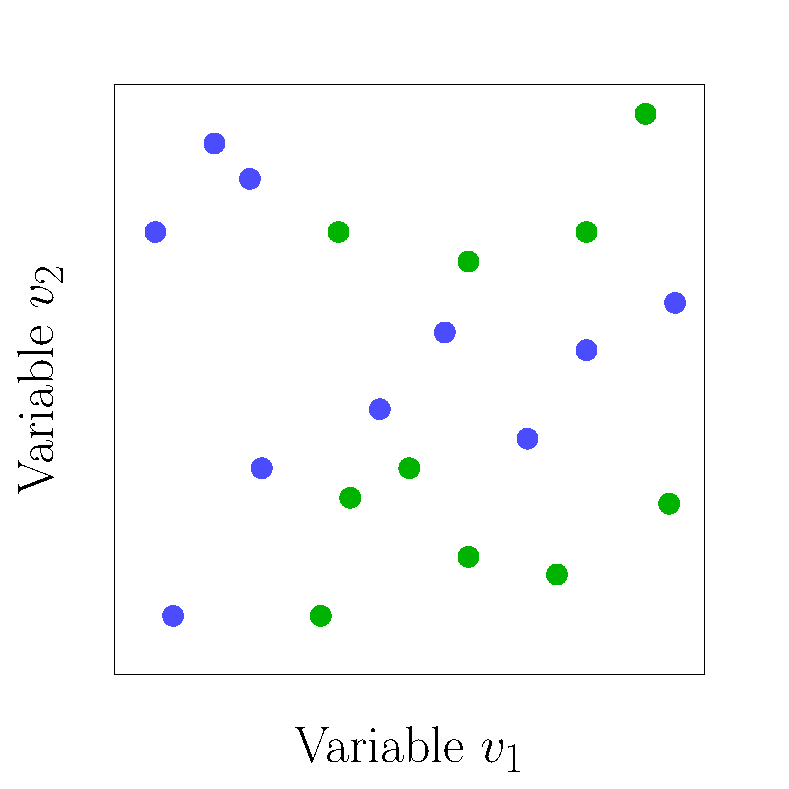
\includegraphics[width=0.45\textwidth]{tikz_rf_dyadique}
        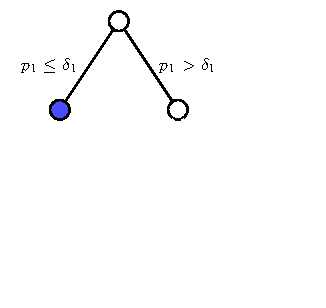
\includegraphics[width=0.45\textwidth]{tikz_rftree_coupure_etape1}
      }
      \only<2>
      {
        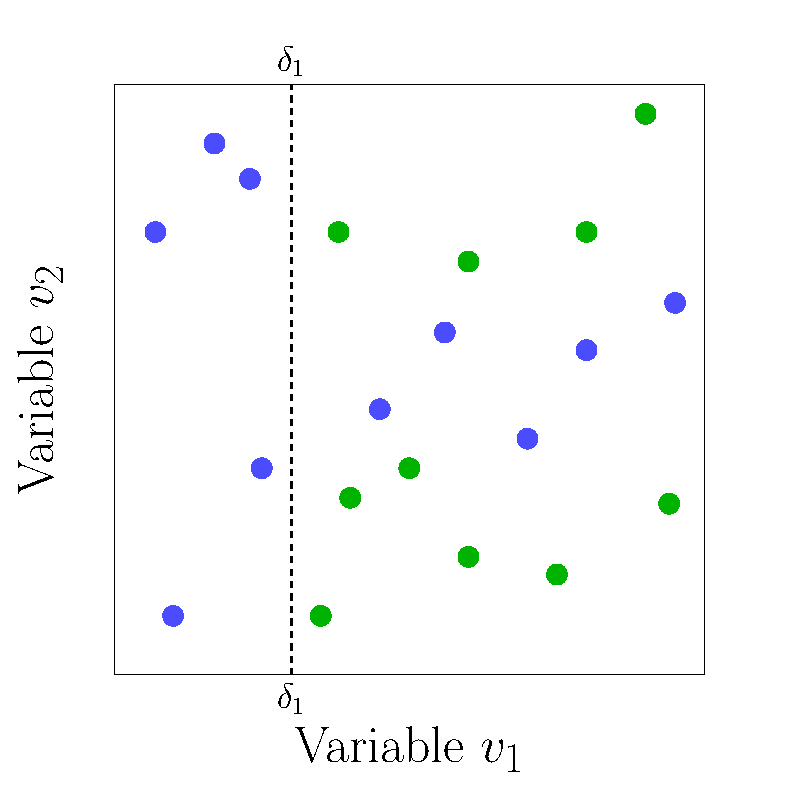
\includegraphics[width=0.45\textwidth]{tikz_rf_dyadique_coupure_etape1}
        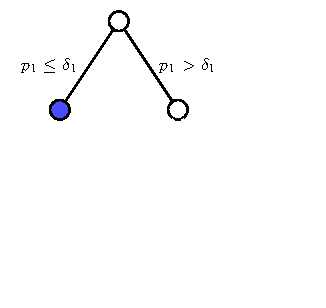
\includegraphics[width=0.45\textwidth]{tikz_rftree_coupure_etape1}
      }
      \only<3>
      {
        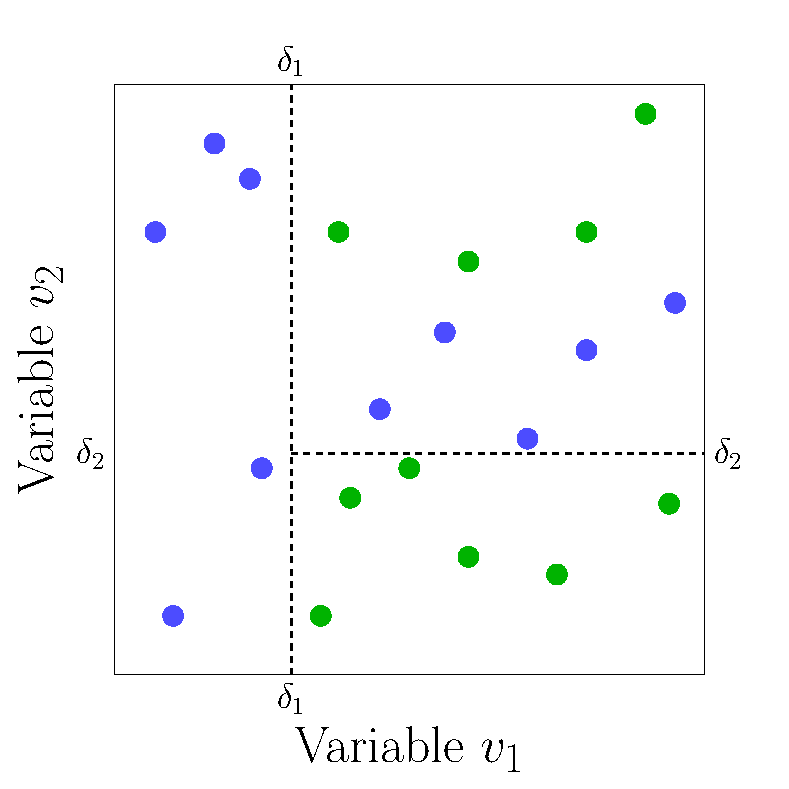
\includegraphics[width=0.45\textwidth]{tikz_rf_dyadique_coupure_etape2}
        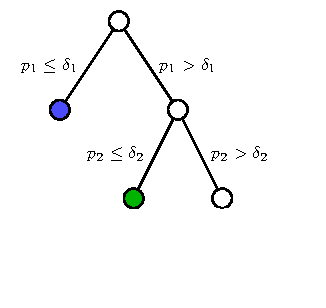
\includegraphics[width=0.45\textwidth]{tikz_rftree_coupure_etape2}
      }
      \only<4>
      {
        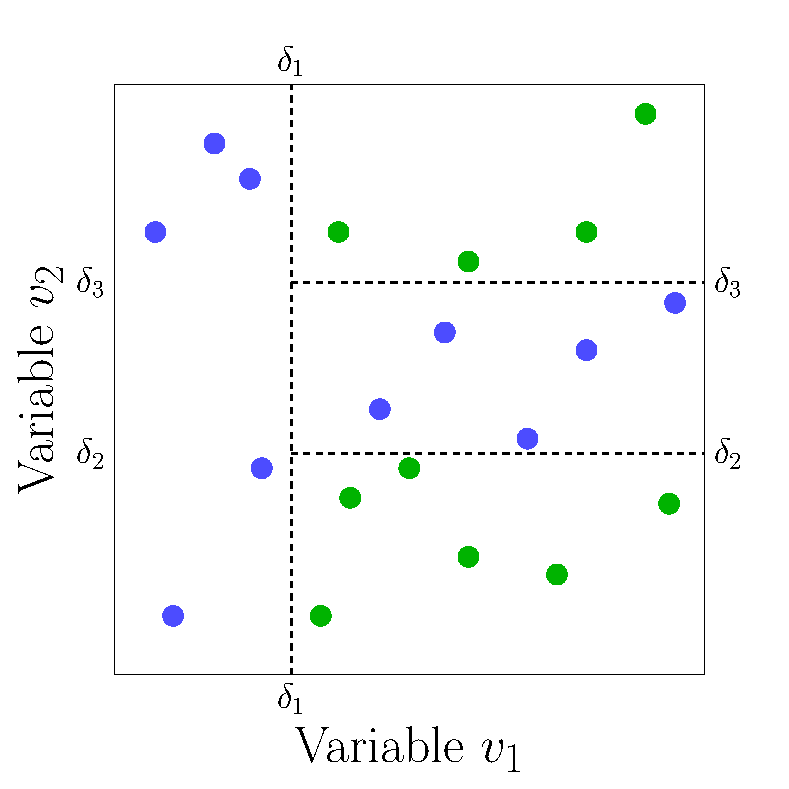
\includegraphics[width=0.45\textwidth]{tikz_rf_dyadique_coupure}
        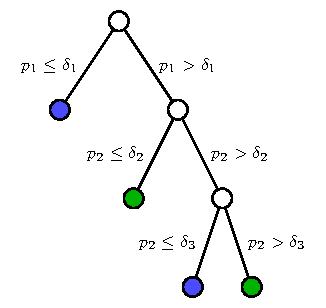
\includegraphics[width=0.45\textwidth]{tikz_rftree_coupure}
      }
    \end{center}
    {\tiny Taken from: Charlotte Pelletier. Cartographie de l’occupation des sols à partir de séries temporelles d’images satellitaires à hautes résolutions Identification et traitement des données mal étiquetées . Interfaces continentales, environnement. Université Toulouse 3 Paul Sabatier (UT3 Paul Sabatier), 2017. Français.}
  \end{frame}

  \begin{frame}{Random Forests}
    \begin{itemize}
    \item For each tree:
      \begin{itemize}
      \item Draw bootstrap sample $X^b$ for training sample
      \item Learn tree, for each node
        \begin{itemize}
        \item select $m$ features from the initial $p$ features
        \item Find the best split (e.g. Gini index, entropy ...)
        \end{itemize}
      \end{itemize}
    \end{itemize}

    \begin{columns}
      \column{0.33\textwidth}
      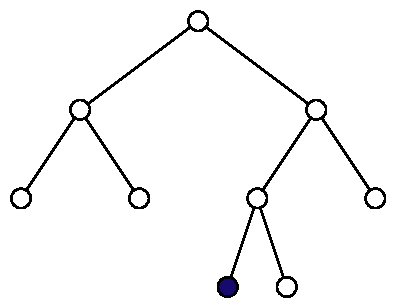
\includegraphics[width=0.95\textwidth]{tikz_rf_outScore_6red.pdf}

      \column{0.33\textwidth}
      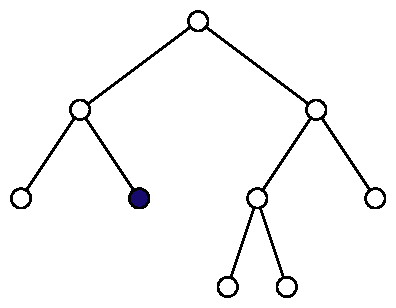
\includegraphics[width=0.95\textwidth]{tikz_rf_outScore_3red.pdf}

      \column{0.33\textwidth}
      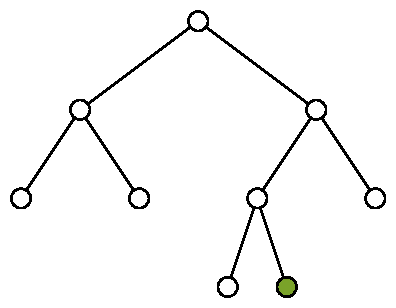
\includegraphics[width=0.95\textwidth]{tikz_rf_outScore_7red.pdf}
    \end{columns}
  \end{frame}

  \begin{frame}{Application: binary data}
    \begin{center}
    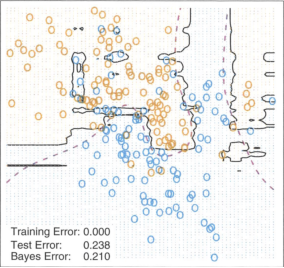
\includegraphics[width=0.55\textwidth]{ex_rf.pdf}
  \end{center}
  \end{frame}

  %\section{Conclusions}
  \begin{frame}
  \frametitle{Conclusions on 'Black Box' approaches}

   \begin{block}{k-NN}
   \begin{itemize}
    \item non-parametric method which does not rely on a fixed model
    \item algorithm which is conceptually  among the simplest of all machine learning algorithms
    \item badly behaved procedure in high dimension: dimension reduction, e.g. PCA, is usually performed prior to k-NN algorithm in order to avoid curse of dimensionality and to reduce computational complexity of the classification rule
   \end{itemize}


   \end{block}


  \begin{block}{SVM}
  \begin{itemize}
   \item maximum margin learning criterion $\leftarrow$ model free
   \item classification algorithm nonlinear in the original input space by performing an implicit linear classification
   in a higher dimensional space
   \item sparse solutions characterized by the support vectors
   \item popular algorithms, with a large literature
    \end{itemize}
 \end{block}

\end{frame}


  \begin{frame}
  \frametitle{Conclusions on 'Black Box' approaches (Cont'd)}

   \begin{block}{ Random Forests}
   \begin{itemize}
    \item involve decision tree to split the prediction space in simple regions
    \item combine multiple decision trees to yield a single consensus prediction
    \item[\doigt] method able to scale efficiently  to high dimensional data
   \end{itemize}
   \end{block}


  \begin{block}{Deep Neural Nets}
  \begin{itemize}
   \item Neural Nets with multiple hidden layers between input and output ones
   \item many variants of deep architectures (Recurrent, Convolutional,...)  used in specific domains (speech, vision, ...)
   \item[\doigt] supported by empirical evidence
   \item[\doigt] dramatic performance jump for several big data applications
    \end{itemize}
 \end{block}

 \alert{Notebook}
\end{frame}


%%% Local Variables:
%%% mode: latex
%%% TeX-master: "main"
%%% End:
